
\documentclass{article}


\usepackage{graphicx}                       % Pacchetti

\usepackage[italian]{babel}

\usepackage{imakeidx}

\usepackage{hyperref}

\usepackage{parskip}

\usepackage{listings}

\usepackage{hyperref}

\usepackage{xcolor}

\lstset{
	showstringspaces=false,
	breaklines=true
}

\usepackage{float}

\usepackage{subfig}


%\usepackage{showframe}



\graphicspath{ {./images/} }

\makeindex[columns=1, title=Tavola dei contenuti, intoc]



\begin{document}

	\begin{titlepage}

		\begin{center}

			\huge\textbf{Montani Website}\\

			\Large\textbf{5 INB}\\

			\Large \textbf{Manuale d'uso}\\

			\vspace{4cm}

			\large Project Manager: \textbf{Boussoufa Yacine}\\

			\large Data: \textbf{02/04/2022}\\

			\large Versione: \textbf{0.1}\\

		\end{center}

	\end{titlepage}

	\clearpage

	\begin{tabular} { |p{1cm}|p{4cm}|p{3cm}|p{2cm}|  }
		

		\hline

			\multicolumn{4}{|c|}{Cronologia delle revisioni} \\

		\hline

		ID & Cambiamenti & Data di creazione & Autore \\

		\hline

		1 & Creazione & 02/04/2022 & Boussoufa \newline Yacine \\

		\hline

	\end{tabular}

	

	\clearpage


	\tableofcontents
	

	\index{generate}

	\clearpage
	

	%Stampa del titolo, autore e data


	\textbf{{\fontsize{5mm}{10mm}\selectfont \section{Introduzione} }}

	\begin{flushleft}
		L'Istituto Tecnico Tecnologico Statale “G. e M. MONTANI” di Fermo ha commissionato una modernizzazione grafica e funzionale del sito web dell'Istituto, il quale non rispetta i requisiti grafici e funzionali, definiti dal modello standard di siti web scolastici realizzato dal Team per la Trasformazione Digitale, su richiesta del Ministero dell’Istruzione.\\
		In riferimento alla Direttiva 8/09 del Ministro per la Pubblica Amministrazione e l'Innovazione, è necessario rispettare quanto specificato all'articolo 4 della direttiva in termini di "Linee Guida per i siti Web della PA" e il "Vademecum". \\
		Il fine di queste linee guida è quello di raggiungere gli obiettivi di gestione, sviluppo e diffusione previsti dalla normativa.\\
	\end{flushleft}

	\vspace{3mm}

	\subsection{\textbf{Interfaccia}}

		Il sito web è stato realizzato attraverso il software di gestione di contenuti (CMS) Wordpress basato su PHP, che permette una gestione facilitata attraverso una dashboard.\\
		Wordpress operando su un web server, e un database, consente la creazione di un sito, formato da contenuti testuali e multimediali, gestibili ed aggiornabili in maniera dinamica: facendo uso di codice HTML, CSS e Javascript.\\
		Wordpress permette anche l'installazione di plugin e temi in modo da personalizzare ulteriormente il sito.

	\vspace{3mm}

	\pagebreak

	\textbf{{\fontsize{5mm}{10mm}\selectfont \section{Wordpress} }}

	\subsection{\textbf{Dashboard}}
	La dashboard di WordPress è la prima schermata che verrà visualizzata dopo aver effettuato l'accesso come amministratore del sito, e permetterà la visualizzazione della panoramica del sito web raccogliendo un vasto numero di gadgets che forniscono le principali informazioni dell'intero sito. La Dashboard può essere personalizzata in base alle esigenze dell'utente e in base ai plugin installati.
	
	\vspace{0.5 cm}

	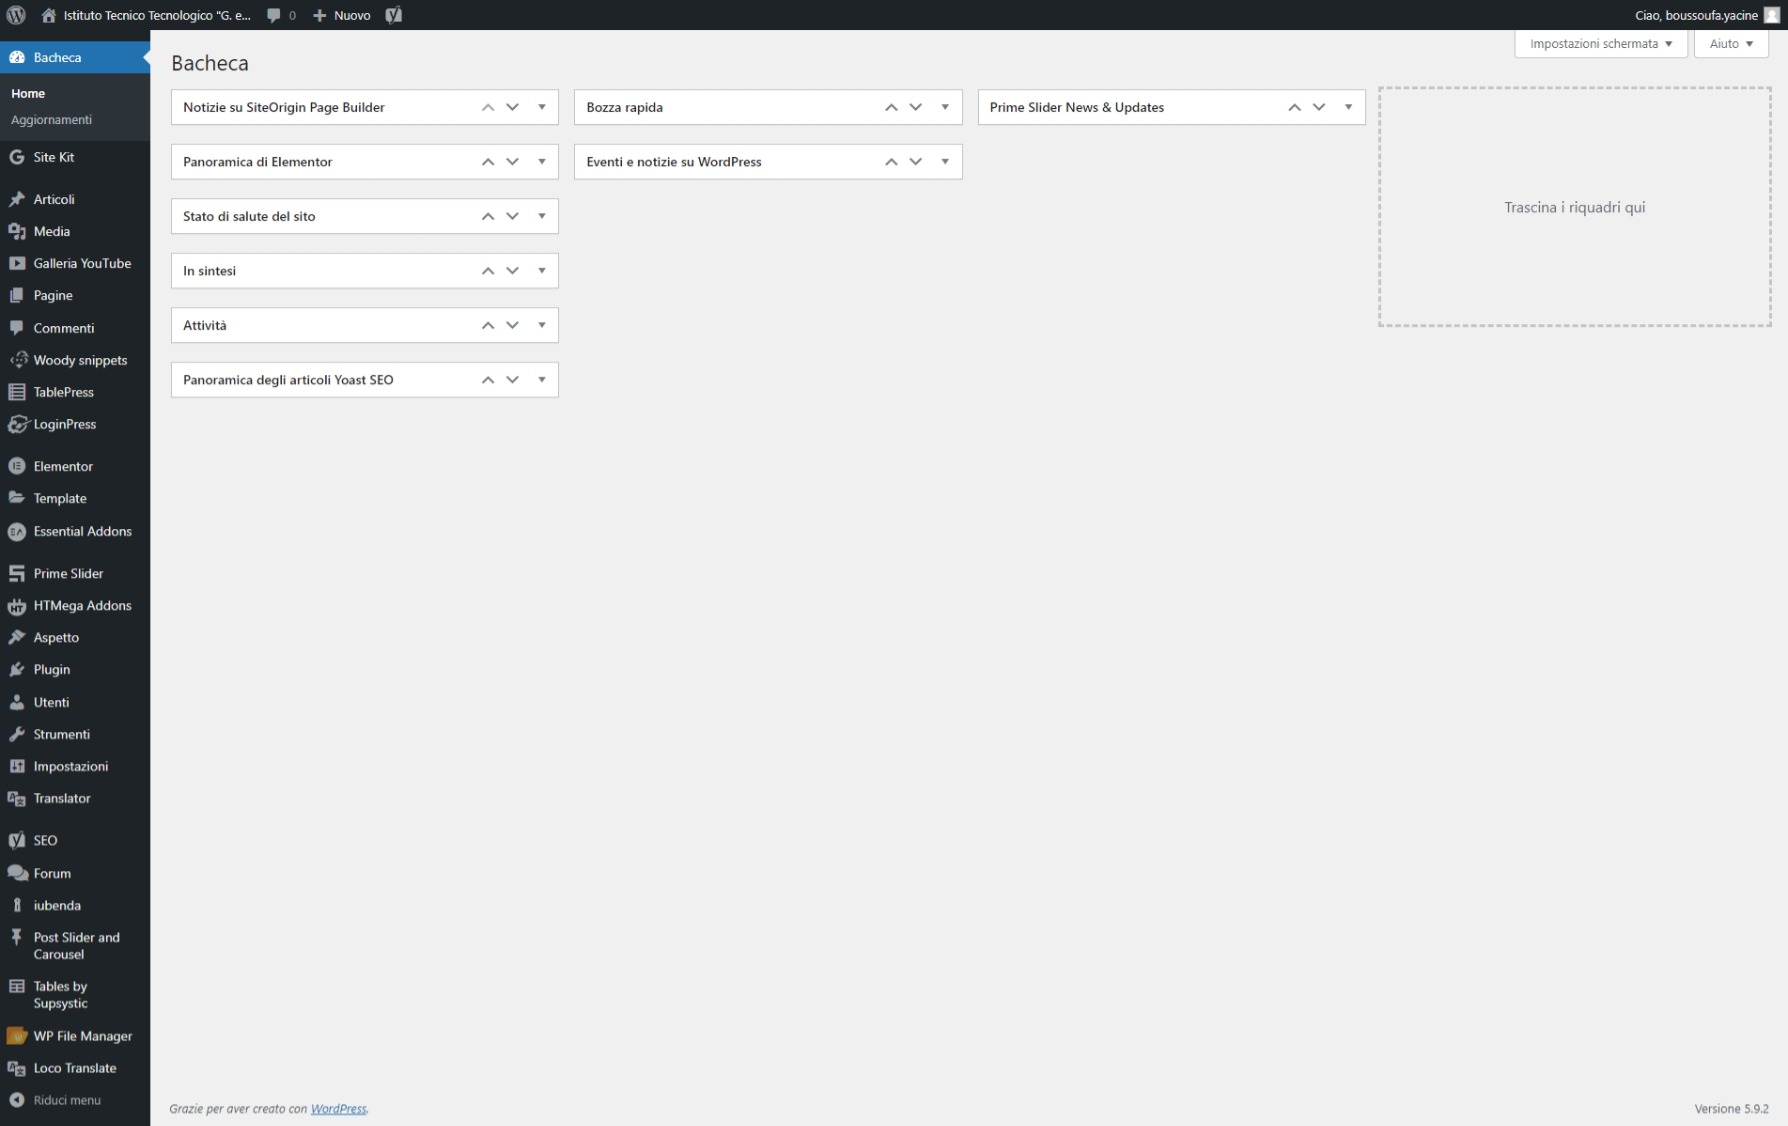
\includegraphics[scale=0.18]{Dashboard Wordpress.jpeg}

	\subsection{\textbf{Tema}}
	Il tema utilizzato per la realizzazione del sito è quello di Designers Italia utilizzabile per i siti internet della Pubblica Amministrazione italiana. (\href{https://github.com/italia/design-wordpress-theme}{Link})\\
	Tuttavia i principali file del tema sono stati modificati manualmente per effettuare alcune correzioni grafiche.\\
	A causa di queste modifiche manuali, non sarà possibile aggiornare il tema in quanto questa operazione sovrascriverà le modifiche effettuate.

	\subsubsection{\textbf{Modificare il tema (Header e Footer)}}
	È quindi possibile modificare il tema utilizzando un client FTP, come FileZilla, e localizzare la cartella al seguente path "/web/wp-content/themes/design-italia/" e modificare a piacimento il codice sorgente.\\
	È inoltre possibile effettuare la modifica direttamente da WordPress:

	\begin{enumerate}
		\item Accedi come amministratore.
		\item Vai nella dashboard principale.
		\item Clicca sulla sezione "Aspetto".
		\item Nel sottomenu clicca su "Editor del tema".
	\end{enumerate}

	La maggior parte dei file modificabili richiedono la conoscenza del linguaggio PHP.	Sarà possibile selezionare il file da modificare dalla barra laterale destra.\\
	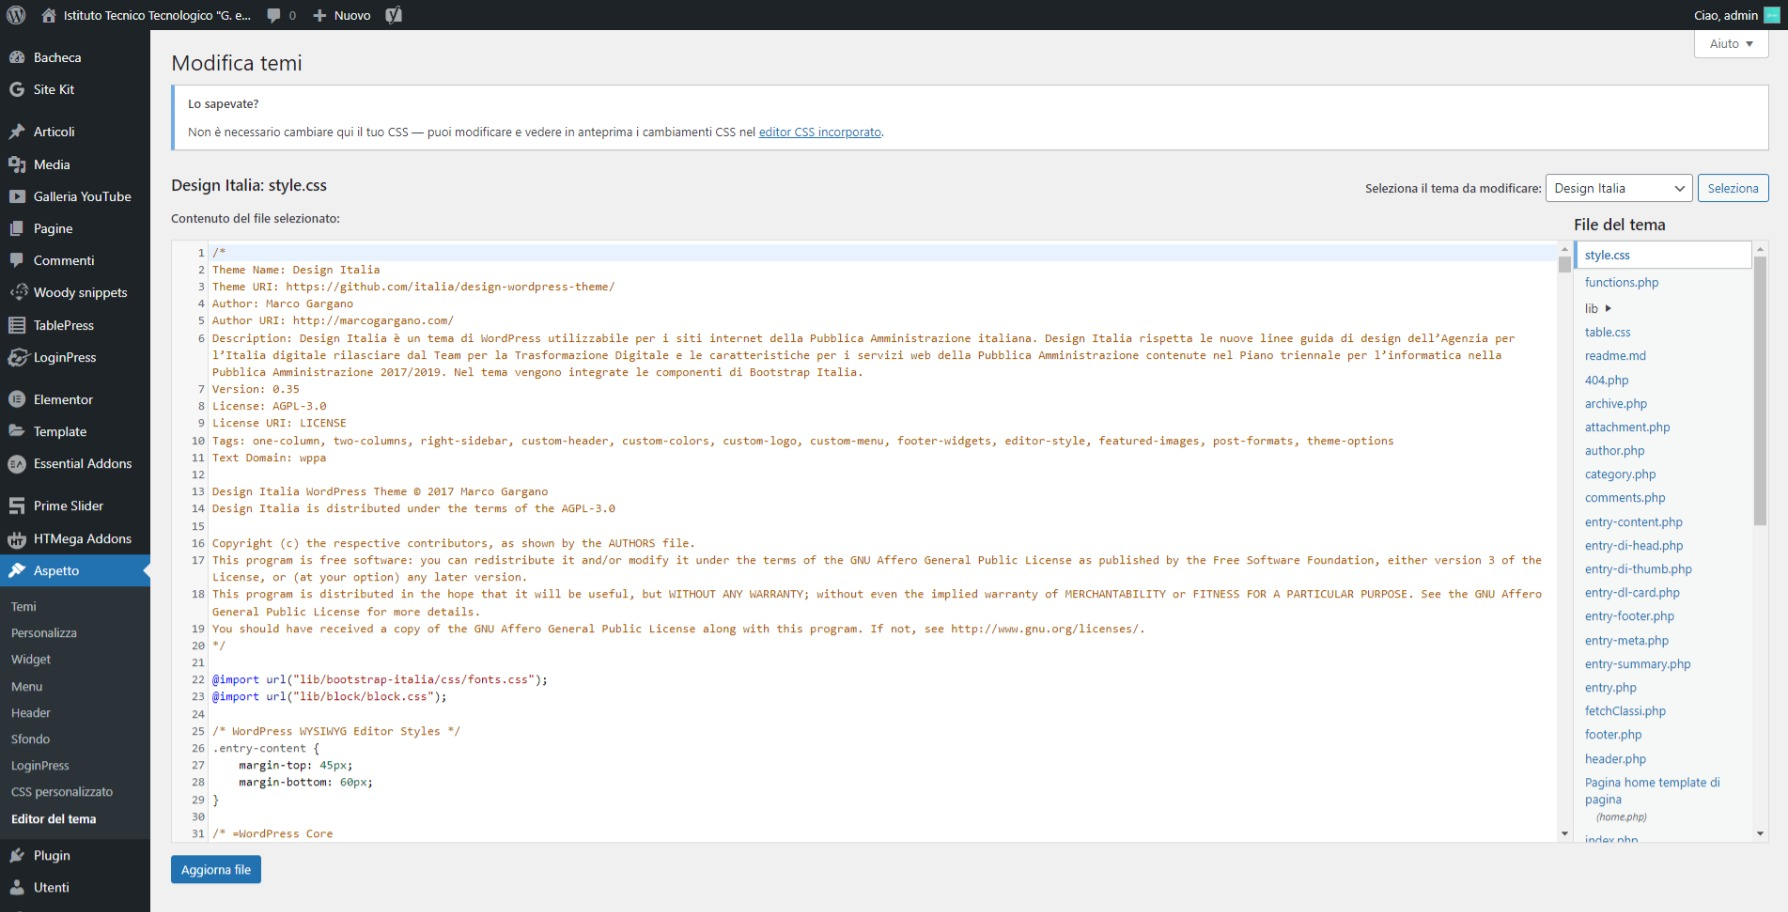
\includegraphics[scale=0.19]{Editor del tema.jpeg}

	\subsubsection{\textbf{Funzioni}}
	All'interno del file "functions.php" sono state create alcune funzioni che possono essere richiamate su wordpress attraverso un blocco denominato shortcode.
	Uno shortcode, è un tag, richiamabile dalle parentesi quadre "[]" e permette di svolgere una particolare funzione all'interno del sito.

	Uno shortcode può essere aggiunto all'interno del file di funzioni come segue:
	\begin{flushleft}
		\begin{lstlisting}[language=php]
function xxxx_shortcode(){
  /* Codice */
}
add_shortcode('xxxx_php_shortcode','xxxx_shortcode');
		\end{lstlisting}
	\end{flushleft}

	ATTENZIONE: non è necessario chiudere il codice PHP.

	\subsubsection{\textbf{CSS aggiuntivo}}
	Per aggiungere del CSS aggiuntivo sarà necessario: 
	\begin{enumerate}
		\item Accedi come amministratore.
		\item Vai nella dashboard principale.
		\item Clicca sulla sezione "Aspetto".
		\item Nel sottomenu clicca su "Personalizza".
		\item Clicca su "CSS aggiuntivo".
		\item Scrivi il nuovo CSS.
	\end{enumerate}

	\subsection{\textbf{Plugin}}
	Per la realizzazione del sito sono stati utilizzati diversi plugin, per questioni di compadibilità, e a causa delle diverse personalizzazioni è consigliato di non aggiornare i plugin.

	\subsection{\textbf{Creazione nuova pagina}}

	Il processo che consente di creare e pubblicare una nuova pagina può essere descritto in base a questi punti chiari e immediati:
	
	\begin{enumerate}
		\item Accedi come amministratore.
		\item Vai nella dashboard principale.
		\item Clicca sulla sezione "Pagine" nel menu laterale sinistro.
		\item Nel sottomenu o nella sezione pagine clicca su "Aggiungi pagina".
		\item Seleziona "Modifica con Elementor".
		\item Lavora sulla nuova pagina. (vedi \hyperref[sec:Elementor]{\textcolor{blue}{sezione Elementor}})
	\end{enumerate}
	In alternativa è possibile creare una pagina, direttamente dalla barra di amministratore presente in alto su tutte le pagine del sito:
	\begin{enumerate}
		\item Accedi come amministratore.
		\item Visualizzare una qualsiasi pagina.
		\item Localizzare la barra di amministrazione in alto.
		\item Effettuare l'hover su " + Nuovo".
		\item Selezionare "Pagina".
		\item Seleziona "Modifica con Elementor".
		\item Lavora sulla nuova pagina. (vedi \hyperref[sec:Elementor]{\textcolor{blue}{sezione Elementor}})
	\end{enumerate}

	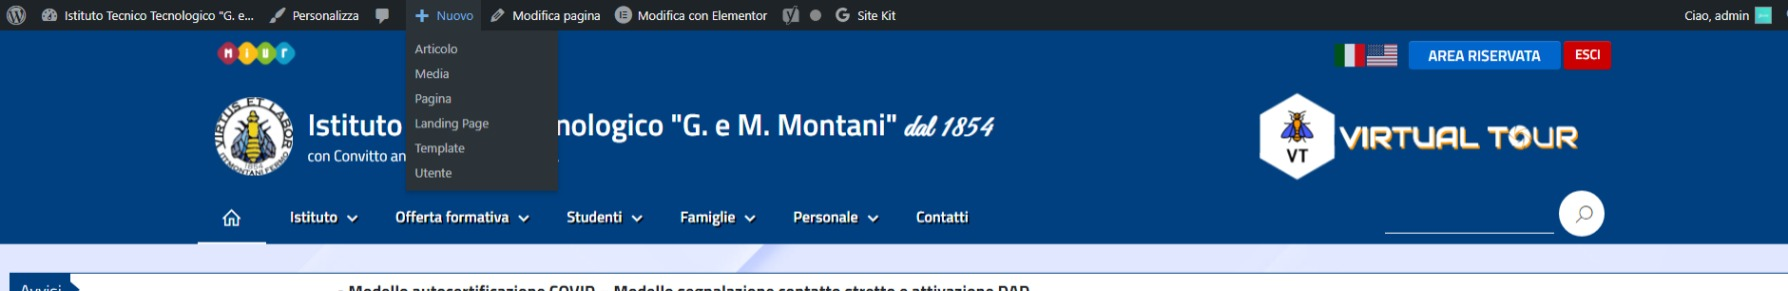
\includegraphics[scale=0.19]{+ Nuovo.jpeg}

	\subsection{\textbf{Creazione di una nuova News (Articolo)}}

	Il processo che consente di creare e pubblicare un nuovo articolo è simile al primo metodo per la creazione di una pagina, tuttavia è necessario prestare maggiore attenzione in modo da semplificare la creazione di un articolo:
	
	\begin{enumerate}
		\item Accedi come amministratore.
		\item Vai nella dashboard principale.
		\item Clicca sulla sezione articoli nel menu laterale sinistro.
		\item Clicca sulla sezione "Tutti gl articoli".
		\item Verrà visualizzata la lista di tutte gli articoli.
		\item Clicca sulla freccia affianco ad "Aggiungi Nuovo".
		\item Clicca su "Editor dei blocchi"
	\end{enumerate}

	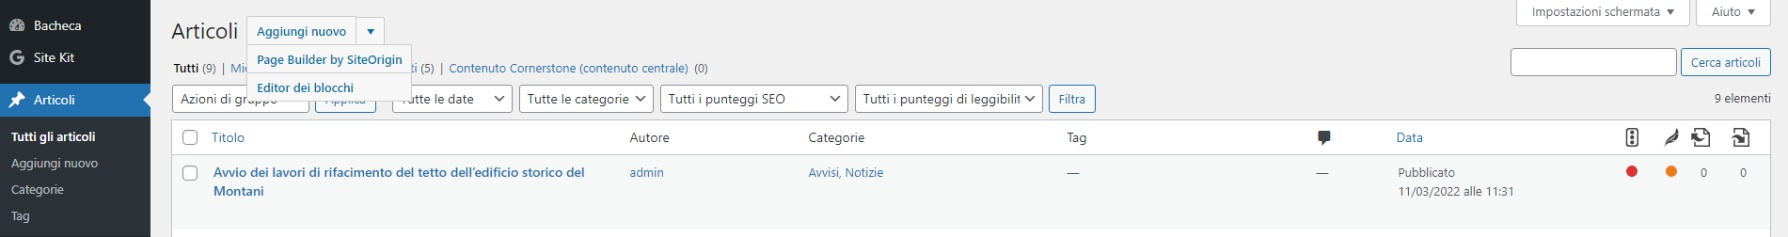
\includegraphics[scale=0.19]{Nuovo Articolo Blocchi.jpeg}

	\textbf{ATTENZIONE}
	\begin{itemize}
		\item NON cliccare dal sottomenu degli articoli "Aggiungi nuovo".
		\item Nel sottomenu "Tutti gli articolI", NON cliccare direttamente "Aggiungi nuovo".
		\item NON effetuare l'hover su "+ Nuovo" nella barra di amministrazione in alto, e cliccare "Articolo".
	\end{itemize}
	Effettuando, i tre punti sopra indicati, non sarà possibile effetuare la modifica utilizzado l'Editor dei blocchi di WordPress, e la modifica di un articolo risulterà più difficoltosa.

	\subsection{\textbf{Editor di Wordpress}}

	Per gli articoli sarà necessario utilizzare l'editor a blocchi di Wordpress. Durante la creazioe e/o modifica sarà presente una barra laterale destra che consentirà di:
	\begin{itemize}
		\item Salvare l'articolo come bozza.
		\item Modificare lo stato di visibilità.
		\item Pubblicare subito, o inserire una data di pubblicazione automatica.
		\item Inserire un'immagine in evidenza.
		\item Selezionare la categoria.
	\end{itemize}

	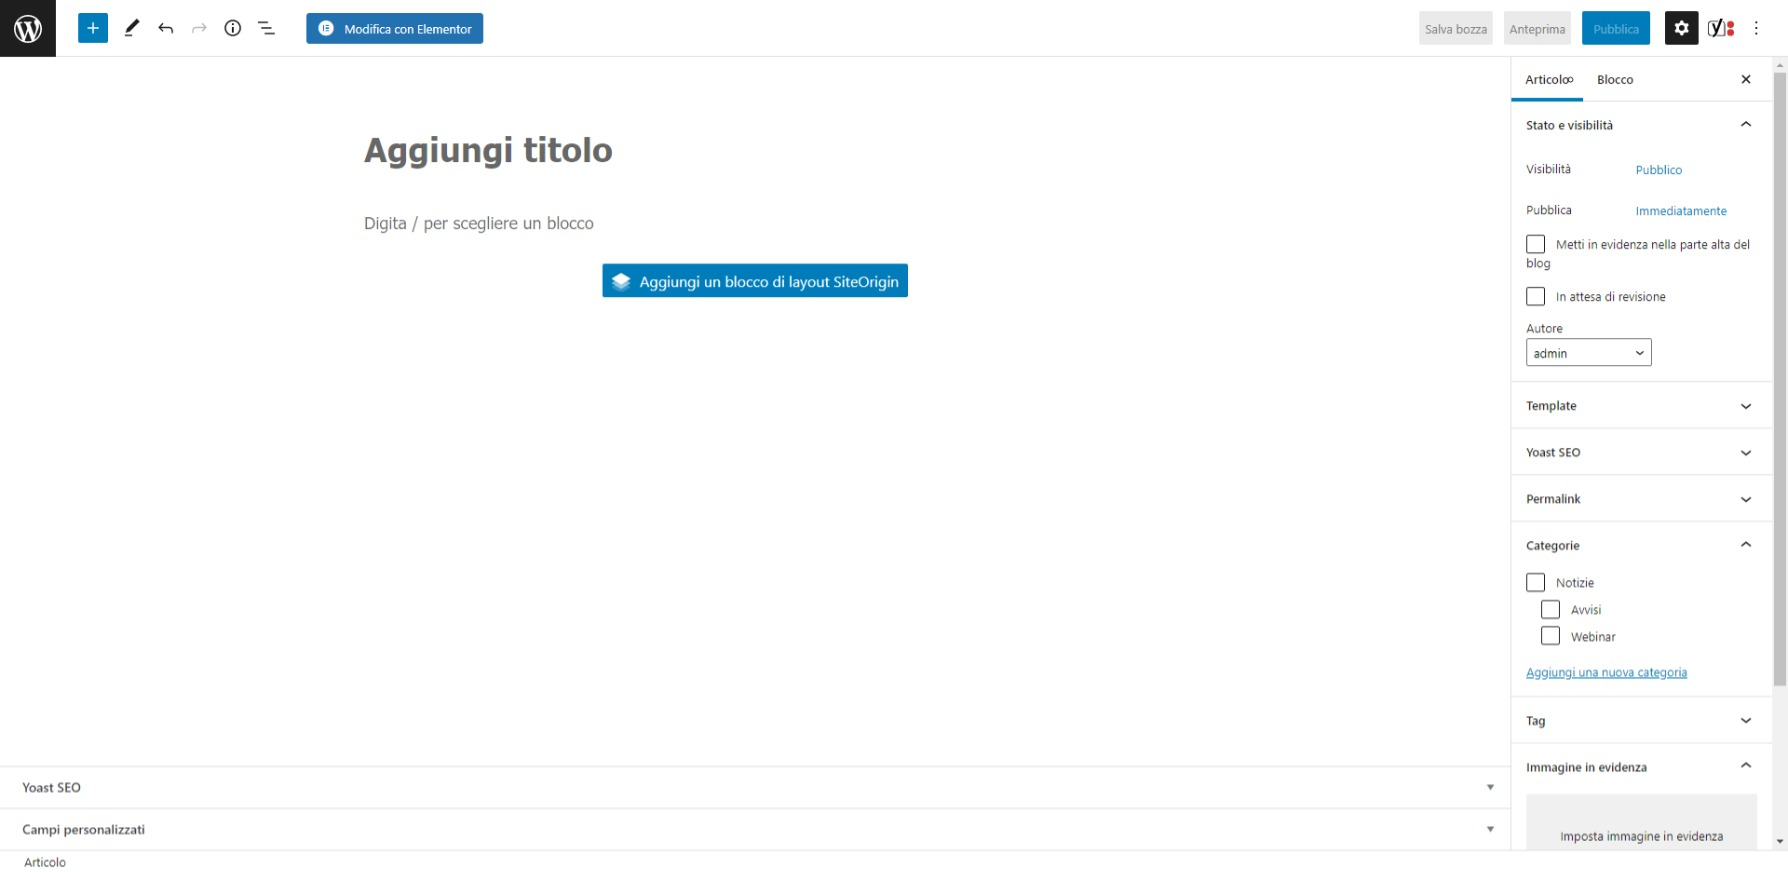
\includegraphics[scale=0.19]{Nuovo articolo.jpeg}

	Per pubblicare un articolo sarà necessario obbligatoriamente, inserire \textbf{un'immagine in evidenza}, che sia di alta qualità; mentre la categoria se non selezionata, verrà automaticamente inserita come "Notizie".\\
	Per inserire un nuovo blocco sarà necessario cliccare il tasto "+" presente a destra, e si raccomanda di \textbf{ignorare il tasto "Aggiungi blocco di layout SiteOrigin"}.\\
	Per inserire un'articolo con la presenza di un video pubblicato su YouTube sarà necessario inserire un blocco HTML ed inserire il seguente codice, in modo da allineare il video al centro della pagina.

	\begin{flushleft}
		\begin{lstlisting}[language=html]
<figure class="wp-block-embed is-type-video is-provider-youtube wp-block-embed-youtube wp-embed-aspect-16-9 wp-has-aspect-ratio">
	<div class="wp-block-embed__wrapper" align="center">
		https://youtu.be/xxxxxxxxxxx
	</div>
</figure>
		\end{lstlisting}
	\end{flushleft}

	\subsection{\textbf{Elementor}}
	\label{sec:Elementor}

	Le pagine dell'intero sito sono realizzate utilizzando un Page Builder denominato 'Elementor': questo ha il vantaggio di poter essere utilizzato senza dover intervenire manualmente su tutto il codice della singola pagina.
	\\Questa tipologia di editor permette di vedere le modifiche al sito man mano che vengono eseguite rendendo più facile e immediata la creazione dell'intero sito.
	\\Procedento alla creazione di una nuova pagina, sarà quindi necessario fare click sul pulsante 'Modifica con Elementor'.

	\vspace{0.5 cm}

	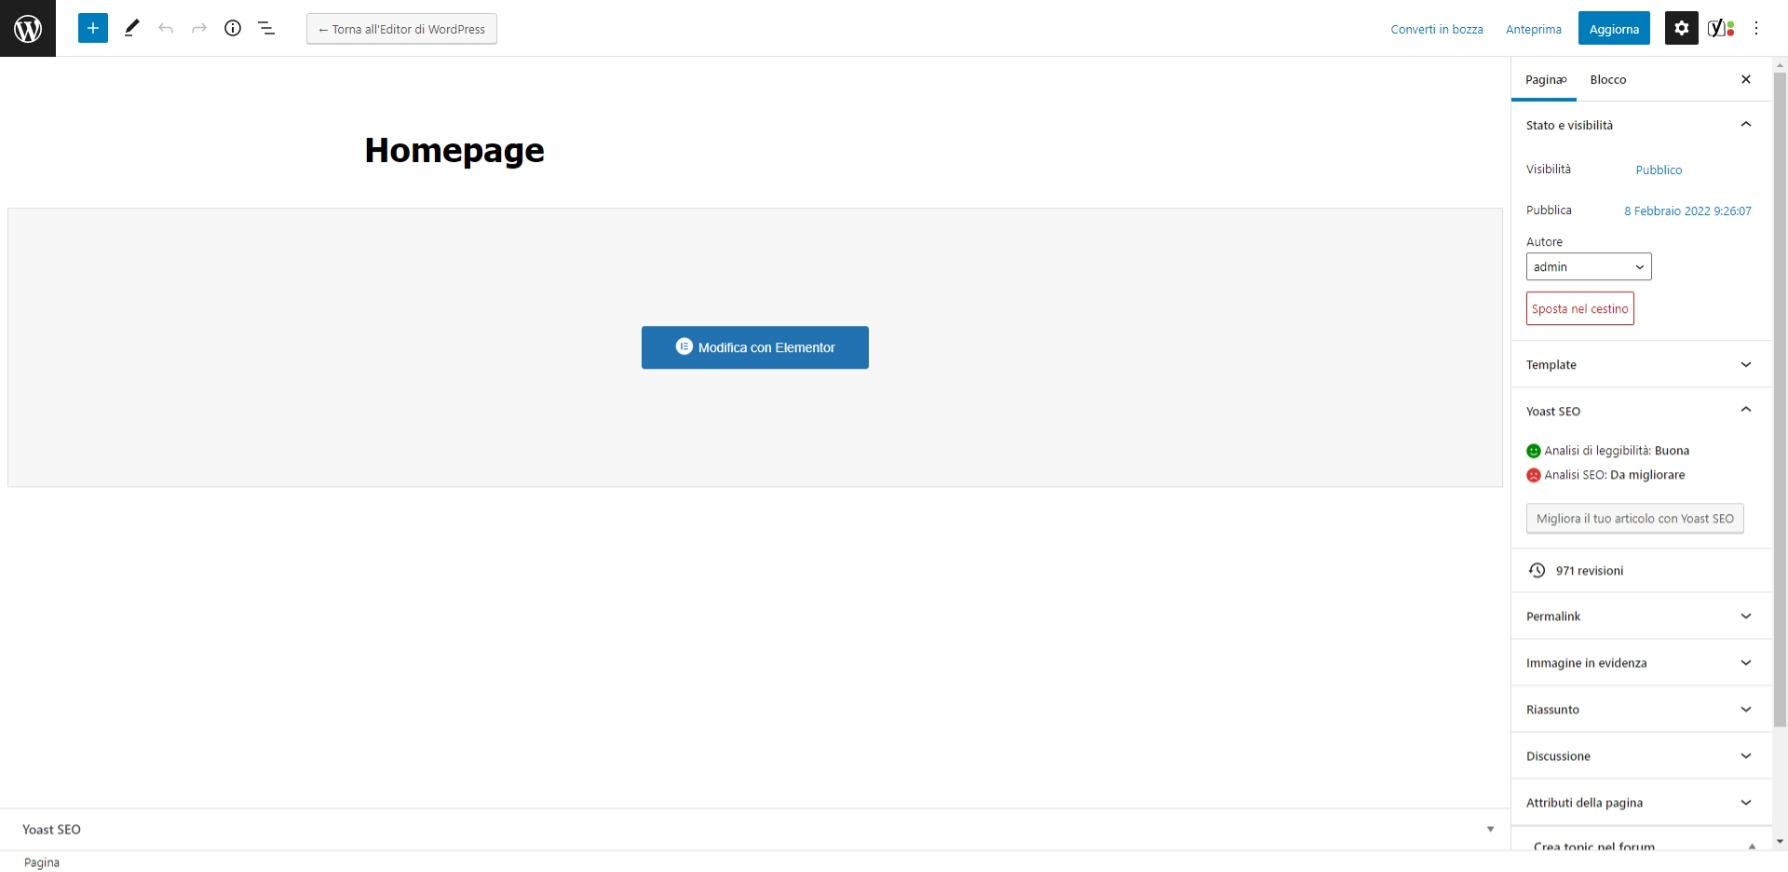
\includegraphics[scale=0.18]{Modifica con Elementor.jpeg}

	\vspace{0.5 cm}

	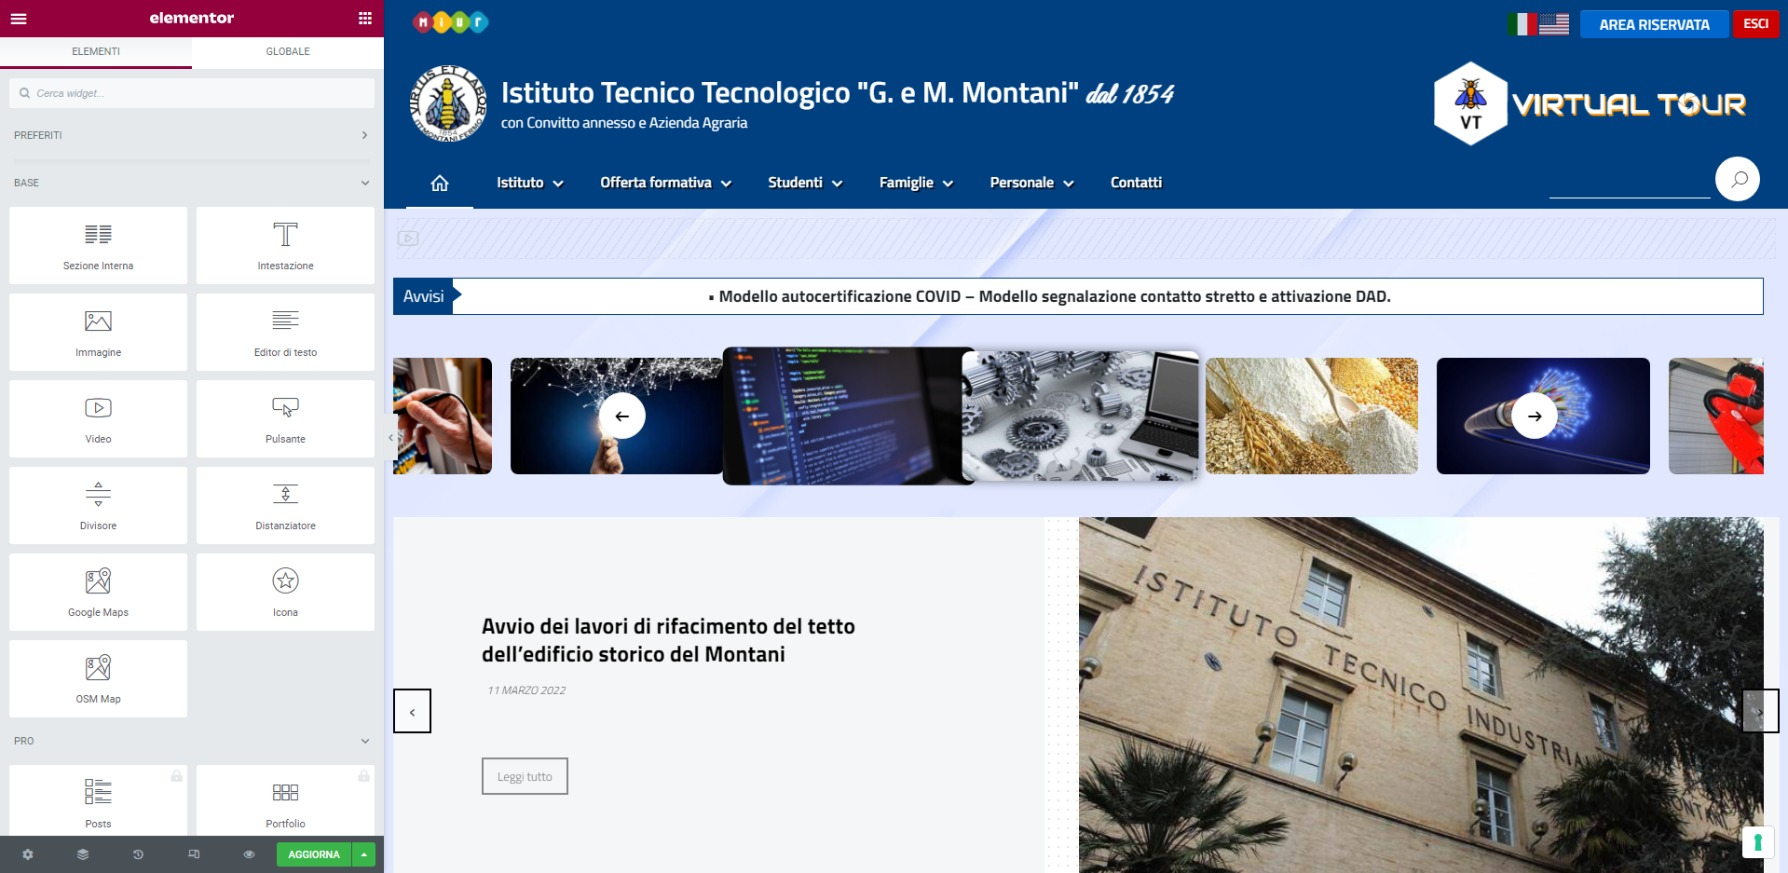
\includegraphics[scale=0.18]{Elementor.jpeg}


	\pagebreak
	
	\textbf{{\fontsize{5mm}{10mm}\selectfont \section{Pagine} }}

	\subsection{\textbf{Homepage}}
	Come sopra indicato, tutte le pagine sono sviluppate attraverso elementor, per questo anche il contenuto della Homepage è stata realizzata utilizzando Elementor ed è strutturato come segue:
	\begin{itemize}
		\item Slider Avvisi;
		\item Slider Indirizzi;
		\item Slider Notizie in evidenza;
		\item Colonna News
		\item Colonna "Servizi"
		\item PON
	\end{itemize}	

	\subsubsection{\textbf{Slider Avvisi}}
		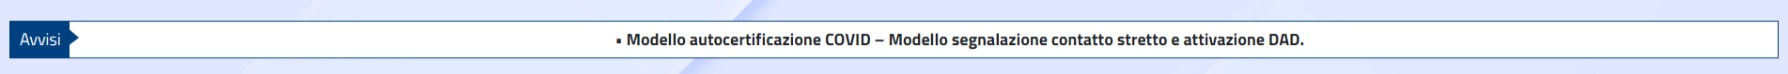
\includegraphics[scale=0.19]{Slider Avvisi.jpeg}\\
		Lo slider degli Avvisi è modificabile attraverso il blocco di Elementor ed è stato generato da codice HTML e da un CSS personalizzato.\\
		Questo codice è modificabile nelle prime righe ed è rappresentato da un'unica lista identificata dal tag 'ul' e da una serie di elementi identificati dal tag 'li'. All'interno di quest'ultimo è presente un collegamento attraverso il tag 'a href' che permete di inserire un testo visualizzabile e un collegamento ipertestuale.\\
	
		\begin{center}
			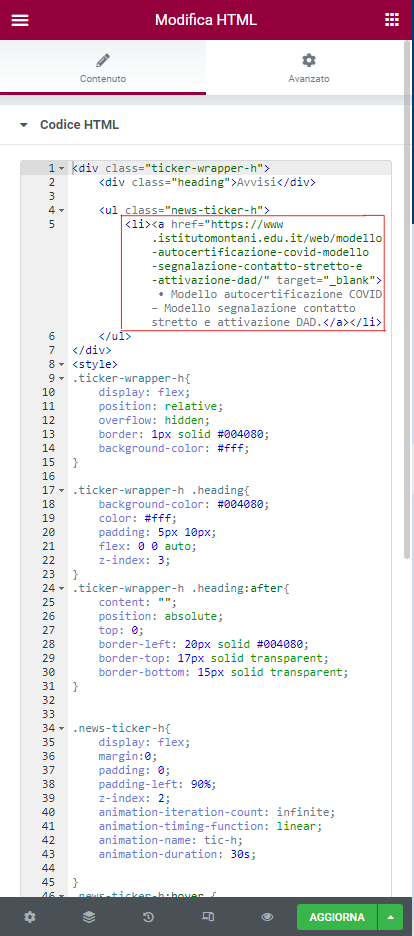
\includegraphics[scale=0.28]{Modifica Slider Avvisi.png}\\
		\end{center}
	\subsubsection{\textbf{Slider Indirizzi}}
		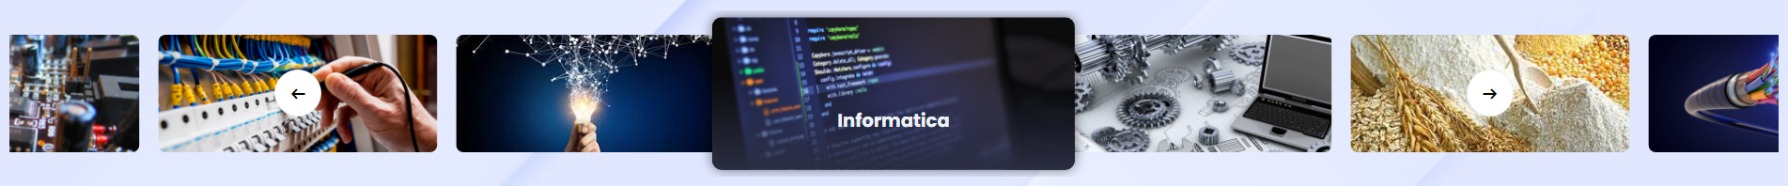
\includegraphics[scale=0.19]{Slider Indirizzi.jpeg}\\
		Lo slider degli indirizzi è inserito su Elementor attraverso l'addon "Prime Slider" utilizzando il blocco Fiestar.\\
		Questo è modificabile effettuando un click con il tasto destro del mouse selezionando "Modifica blocco".
		Elementor permette, nelle varie sue impostazioni, di modificare il contenuto al suo interno attraverso alcune query che richiamano le pagine esistenti nel sito, e permette anche la modifica dello stile grafico.\\
		Le immagine delle pagine sono quelle caricate come "immagini in evidenza" della singola pagina, presente nell'editor predefinito di Wordpress. 

		\vspace{0.2 cm}
		\begin{center}
			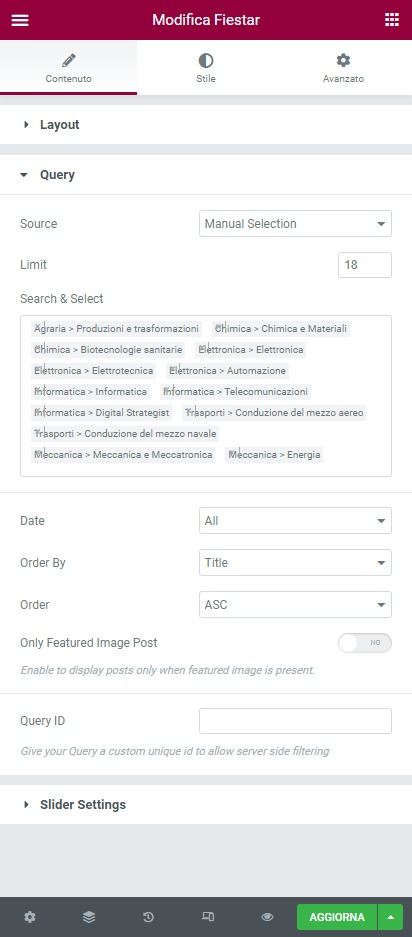
\includegraphics[scale=0.28]{Modifica Slider Indirizzi.jpeg}\\
		\end{center}
	\subsubsection{\textbf{Slider Notizie in evidenza}}
	Lo slider delle principali notizie è gestito separatamente da telefono e da pc.
	In particolare il primo è gestito da un plugin, mentre il secondo da uno shortcode di un secondo plugin.
	
	Per PC lo slider sarà generato dal seguente shortcode: 
	

[psac\_post\_slider design="design-2" show\_author="false" show\_comments="false" show\_category="false" show\_content="true" autoplay\_interval="5000"\\ speed="500" category="Avvisi"]

	Per Mobile è stato utilizzato un plugin modificabile da elementor. Per inserire il plugin sarà necessario cliccare sul "+" per una nuova sezione e selezionare la cartella grigia. Selezionare poi "Template Personalizzati" e inserire i due template sia da PC che da Mobile.
	ATTENZIONE: Selezionare sempre NO in caso di comparsa di un Pop-Up. I plugin risulteranno invisibili (vuoti) se nella categoria associata non esistono articoli.
	
	Per modificare gli slider:
	Per il PC: andare in bacheca, scorrere in basso, localizzare nella barra laterale destra "Post Slider Carousel" e generare uno shortcode in base alle proprie esigenze.
	Per mobile: selezionare il widget dalla modifica di Elementor, e personalizzare nella sezione Query.

	ATTENZIONE: nel plugin per PC è possibile inserire solo categorie e non articoli singoli, sarà quindi necessarrio creare una categoria ed aggiungere gli articoli prescelti, per poi modificare lo shortcode con category="xxxx".

	\subsubsection{\textbf{Colonna News}}
	La griglia degli articoli è generata automaticamante attraverso il Widget di SiteOrigin e sviluppato da Designers Italia: modificandolo sarà possibile, cambiare il numero di articoli in totale, selezionare la categoria degli articoli (predefinita: Notizie), e modificare altre opzioni di visualizzazione.
	Per una questione di spazio il titolo è stato limitato a quattro righe, attraverso l'utilizzo di un CSS personalizzato.
	\begin{center}
		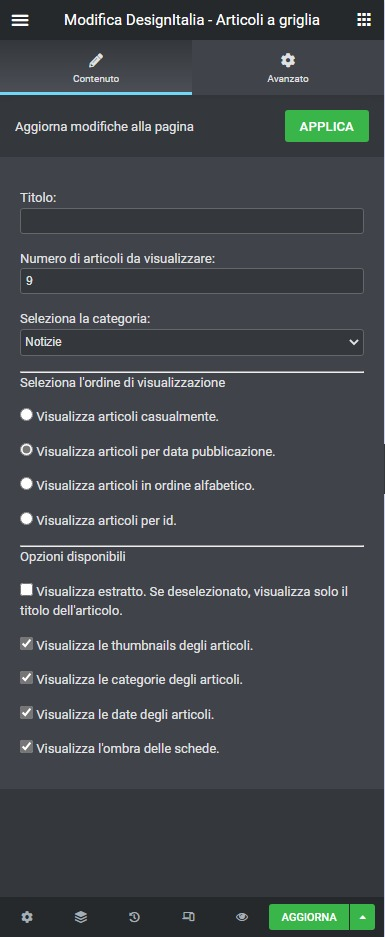
\includegraphics[scale=0.2]{Modifica articoli a griglia.jpeg}
	\end{center}

	\subsubsection{\textbf{Colonna "Servizi"}}
	I riquadri dei servizi sono rappresentati dal blocco "Service" di Elementor a cui è inserito come contenuto, un'immagine e un link ipertestuale.\\
	Per uniformare la grandezza di tutti i riquadri, nella sezione "Stile", più precisamente su Image è stato modificato il margine di tutte le immagini.

	\begin{figure}[H]%
		\centering
		\subfloat{{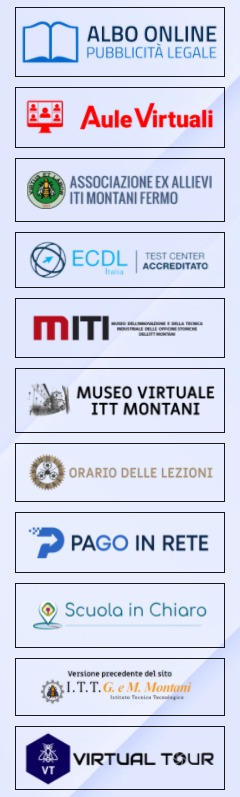
\includegraphics[scale=0.235]{Servizi.jpeg} }}
		\qquad
		\subfloat{{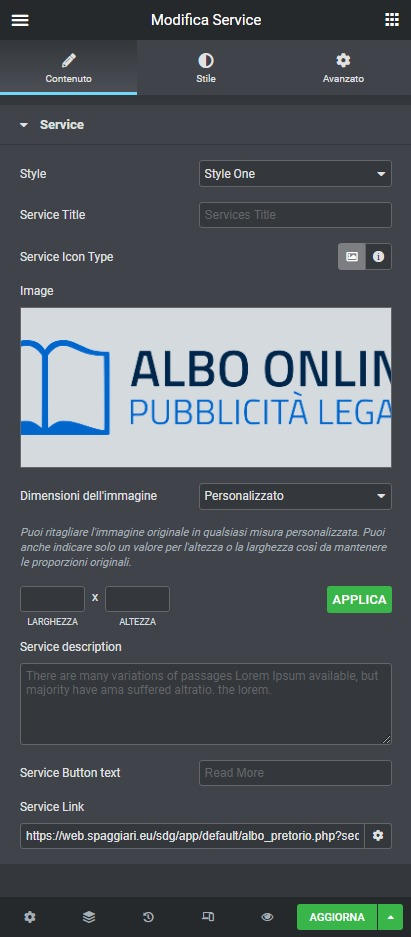
\includegraphics[scale=0.2]{Blocco servizi.jpeg} }}
		\label{fig:example}%
	\end{figure}

	\subsubsection{\textbf{PON}}
	Il logo del PON è inserito come semplice immagine, al suo interno è presente un collegamento ipertestuale che reindirizza a una pagina all'interno del sito.

	\vspace{0.2 cm}
	
\includegraphics[scale=0.2]{PON.jpeg}

	\subsubsection{\textbf{Nascondere/Mostrare un contenuto}}
	Per nascondere e mostrare un contenuto già nascosto, bisognerà accedere alle impostatazioni avanzate di un widget e localizzare la sezione "Responsive".
	Sarà poi necessarrio attivare i tick (colore azzurro) per nascondere i contenuti sui vari dispositivi. E disattivarli (grigi) per mostrarli.

	\subsection{\textbf{Forum}}
	Il forum è gestito attraverso il plugin Asgaros Forum. Ed è modificabile attraverso le impostazioni del plugin.
	Attraverso una funzionalità del plugin sono stati creati 2 ruoli (Utenti e Docenti) i quali vengono assegnati con la stessa procedura dei permessi Wordpress.
\pagebreak
	\subsection{\textbf{Indirizzi}}
	Le pagine d'indirizzo sono composte da un widget di elementor suddiviso in 4 schede con:
	\begin{itemize}
		\item Descrizione: campo testuale con descrizione.
		\item Tabelle: 
		\item Progetti: Per i progetti sono state definite delle funzioni nel file functions.php le quali gestiscono:\\ caricamento \begin{verbatim}progetti_insert_shortcode\end{verbatim} modifica \begin{verbatim}progetti_modify_shortcode\end{verbatim} visualizzazione nella pagina d'indirizzo \begin{verbatim}progetti_query_shortcode\end{verbatim} visualizzazione dei progetti dell'utente \begin{verbatim}progetti_display_shortcode\end{verbatim} visualizzazione completa del singolo progetto \begin{verbatim}progetti__shortcode\end{verbatim} eliminazione del progetto \begin{verbatim}progetti_delete_shortcode\end{verbatim}
		\item Galleria Foto: per la galleria foto è stata scritta una funzione in functions.php \begin{verbatim}
		immagini_shortcode
		\end{verbatim} la quale prende il nome della pagina (es. informatica) e legge e visualizza tutte le immagini  presenti nel path \begin{verbatim}/web/wp-content/uploads/img_indirizzi/<nomepagina>\end{verbatim} Per aggiungerne basterà rilasciare le immagini nella specifica cartella.
	\end{itemize}


	\subsection{\textbf{Webinar}}
	
	\subsection{\textbf{Repository}}
	Per le funzionalità di repository è stato progettato un ampliamento del database di Wordpress. Per interfacciarsi con esso sono state definite delle funzioni nel file functions.php del tema le quali leggono, modificano, inseriscono e rimuovono dati attraverso le query. Per richiamare in una pagina una funzione presente nel file functions.php vengono utilizzati gli shortcode, i quali vengono anch'essi definiti nel medesimo file.
		\subsubsection{\textbf{Libri di Testo}}
		Per i libri di testo sono state definite le seguenti funzioni:
		\begin{itemize}
			\item \begin{verbatim}
			libritesto_insert_shortcode
			\end{verbatim}: utilizzata per il caricamento di nuovi libri di testo nel database.
			Il corrispondente shortcode è \begin{verbatim}libritesto_php_input\end{verbatim}
			\item \begin{verbatim}
			libritesto_query_shortcode
			\end{verbatim}: utilizzata per mostrare i libri di testo dal database. Necessita dell'anno scolastico e l'anno di corso come parametri in get. Il corrispondente shortcode è \begin{verbatim}
			libritesto_php_output
			\end{verbatim}
			\item \begin{verbatim}
			libritesto_display_shortcode
			\end{verbatim}: utilizzata per mostrare i libri di testo di un utente dal database. Il corrispondente shortcode è \begin{verbatim}
			libritesto_php_display
			\end{verbatim}
			\item \begin{verbatim}
			libritesto_delete_shortcode
			\end{verbatim}: utilizzata per rimuovere i libri di testo di un utente dal database. Il corrispondente shortcode è \begin{verbatim}
			libritesto_php_delete
			\end{verbatim}
		\end{itemize}
		\subsubsection{\textbf{Modulistica}}
		Per la modulistica sono state definite le seguenti funzioni:
		\begin{itemize}
			\item \begin{verbatim}
			modulistica_insert_shortcode
			\end{verbatim}: utilizzata per il caricamento di nuova modulistica nel database.
			Il corrispondente shortcode è \begin{verbatim}
			modulistica_php_input
			\end{verbatim}
			\item \begin{verbatim}
			modulistica_query_shortcode
			\end{verbatim}: utilizzata per mostrare la modulistica dal database. Il corrispondente shortcode è \begin{verbatim}
			modulistica_php_output
			\end{verbatim}
			\item \begin{verbatim}
			modulistica_display_shortcode
			\end{verbatim}: utilizzata per mostrare la modulistica di un utente dal database. Il corrispondente shortcode è \begin{verbatim}
			modulistica_php_display
			\end{verbatim}
			\item \begin{verbatim}
			modulistica_delete_shortcode
			\end{verbatim}: utilizzata per rimuovere la modulistica di un utente dal database. Il corrispondente shortcode è \begin{verbatim}
			modulistica_php_delete
			\end{verbatim}
		\end{itemize}
		\subsubsection{\textbf{Programmazioni}}
		Per la programmazioni sono state definite le seguenti funzioni:
		\begin{itemize}
			\item \begin{verbatim}
			programmazioni_insert_shortcode
			\end{verbatim}: utilizzata per il caricamento di nuove programmazioni nel database.
			Il corrispondente shortcode è \begin{verbatim}
			programmazioni_php_input
			\end{verbatim}
			\item \begin{verbatim}
			programmazioni_query_shortcode
			\end{verbatim}: utilizzata per mostrare le programmazioni dal database. Il corrispondente shortcode è \begin{verbatim}
			programmazioni_php_output
			\end{verbatim}
			\item \begin{verbatim}
			programmazioni_display_shortcode
			\end{verbatim}: utilizzata per mostrare le programmazioni di un utente dal database. Il corrispondente shortcode è \begin{verbatim}
			programmazioni_php_display
			\end{verbatim}
			\item \begin{verbatim}
			programmazioni_delete_shortcode
			\end{verbatim}: utilizzata per rimuovere le programmazioni di un utente dal database. Il corrispondente shortcode è \begin{verbatim}
			programmazioni_php_delete
			\end{verbatim}
		\end{itemize}
	

	\pagebreak

\end{document}